\chapter{Metode}
\textit{I dette kapitel beskrives formålet med udviklingen af et system til risikovurdering af lægemiddelskift, udviklingsprocessen, herunder dataindsamling, udvælgelse af risikofaktorer og deres vægtning, præprocessering, design, implementering og test samt evaluering af systemet.}

\section{Formål}
Formålet er at udvikle et regelbaseret system til risikovurdering af lægemiddelskift med henblik på at evaluere anvendeligheden af systemet. For at undgå at vurderingen af implementering af lægemiddelskift er personafhængig og sårbar, som den er på nuværende tidspunkt, udvikles et system, som sammenligner flere risikofaktorer fra forskellige databaser, hvilket den menneskelige evne ikke er tilstrækkelig til. Systemet foretager en risikovurdering ud fra risikofaktorer, som er vægtet af en ekspert på området, i forhold til at vurdere hvor kompleks implementering af lægemiddelskift er. Ud fra risikovurderingen skal det være muligt for ATC-ansvarlige medarbejdere at udarbejde Lægemiddel Nyt, som fremgår af Appendiks~\ref{cha:AppD}, punktnummer \ref{item:Laegemiddelnyt}. Lægemiddel Nyt sendes ud til de enkelte hospitalsafdelinger med henblik på at rådgive i forhold til hvilke lægemiddelskift der skal være særligt opmærksomme på i forbindelse med implementeringen for at forebygge medicineringsfejl og derved forbedre patientsikkerheden. 

\section{Udviklingsproces}
Udviklingen af et system til risikovurdering af lægemiddelskift gennemgår forskellige udviklingstrin, herunder indsamling af data, udvælgelse af risikofaktorer og vægtning af disse, præprocessering af data, design, implementering og test samt evaluering af systemet. Udviklingsprocessen har foregået som en iterativproces, hvor der har været overlap mellem de enkelte trin. Udviklingstrinene fremgår af Figur \ref{fig:metode}. 

\begin{figure}[H]\centering	\includegraphics[width=1\textwidth]{billeder/udviklingstrin.png} 
	\caption{Udviklingstrin for processen.}
	\label{fig:metode}  
\end{figure}
\vspace{-0.5cm}

Af Figur \ref{fig:metode} illustreres de forskellige udviklingstrin som gennemgås ved udviklingen af et system til risikovurdering af lægemiddelskift. Indsamling af data danner grundlaget for den næste proces i forhold til udvælgelse af risikofaktorer. Risikofaktorer er udvalgt på baggrund af indsamlet data og litteratur. Disse vægtes efterfølgende af en ekspert inden for området. Dernæst foretages præprocessering af data for at gøre data homogent og sammenligneligt. Efterfølgende designes systemet som omhandler design af risikovurdering. Herefter implementeres designet af systemet. De enkelte dele af systemet er løbende testet og valideret i forhold til systemet performans. Til sidst evalueres systemet i forhold til brugervenlighed og fremtidige forbedringer. 
%Udvælgelsen af risikofaktorer danner grundlag for de inputs som vægtes i forhold til risikovurderingen. Da data ikke er homogen ønskes det at foretage præprocessering af data for at gøre data sammenligneligt. Designfasen bygger på design af algoritmen som danner grundlag for risikovurderingen. Designet verificeres i løbet af processen for at opnå det bedst mulige design. Herefter implementeres systemet, hvilket omfatter implementering af designet herunder kodning af regel-baseret ekspert system. Til sidst foretages en test af systemet i forhold til evaluere hvorvidt systemet performer efter formålet, hvis dette ikke er tilfældet vendes der tilbage til de fortgående udviklingstrin i forhold til at omformulere i  præprocessingsfasen, redesigne i systemet i designfasen eller tilpasse kodningen i implementeringensfasen. 


%med henblik på at gøre den nuværende vurdering af kompleksiteten af lægemiddelskift mindre personafhæning og sårbar. 
%Den nuværende risikovurdering af kompleksiteten af implementering af lægemiddelskift varetages af ATC-ansvarlige på baggrund af tidligere erfaringer, retningslinjer, indsamlede problemstillinger vedrørende lægemiddelskift samt viden omkring lægemidler indsamlet via f.eks. pro.medicin. ATC-områderne er uddelt på de forskellige ATC-ansvarlige, så hver ATC-ansvarlig har hvert deres område. I vurderingen af lægemiddelskiftet vægtes risikofaktorer, som f.eks. ændring i navn, styrke og dispenseringsform, af én ATC-ansvarlig for området, hvormed denne proces er personafhængig og stiller visse krav til den ATC-ansvarliges viden og erfaring inden for området. Vægtningen udføres i forhold til at vurdere risikoen ved implementering af lægemiddelskift på hospitalsafdelingerne. Ud fra vægtningen udarbejdes et Lægemiddel Nyt Tema omkring skiftet, hvilket fremgår af Appendiks \ref{cha:AppD} nummer \ref{item:Laegemiddelnyt}. Dette udarbejdes med henblik på at synliggøre i hvilke tilfælde hospitalsafdelingerne skal være særlig opmærksomme på lægemiddelskiftet i forhold til at undgå fejlmedicinering som f.eks. kan forårsages af forveksling ved ændringer i lægemiddelnavn.
%For at imødekomme disse problemstillinger ønskes det at udvikle et computerbaseret system til risikovurderingen af lægemiddelskift, som gør den nuværende proces mindre personafhængig, samt vurderer flere risikofaktorer og derved danner et bedre grundlag for den ATC-ansvarlige i forbindelse med risikovurderingen af lægemiddelskiftet. 


%På nuværende tidspunkt vurderes kompleksiteten af implementering af lægemiddelskift af ATC-ansvarlige ud fra tidligere erfaringer og viden indsamlet via bl.a. pro.medicin. Flere faktorer vægtes ved vurderingen, hvilket gør denne proces meget personafhængig og stiller visse krav til den ATC-ansvarliges viden og erfaring inden for området. Vurderingen der foretages har betydning for implementeringen af lægemiddelskiftet i klinikken og det er derfor vigtigt at den rette vurdering foretages i forhold til at undgå medicineringsfejl som f.eks. forveksling af navnet på lægemidlet grundet ændringer ved lægemiddelskift. For at imødekomme disse problemstillinger ønskes det at udvikle et beslutningsstøttesystem til den ATC-ansvarlige som foretager risikovurderingen af lægemiddelskift med henblik på at synliggøre de ændringer som sker ved et eventuelt lægemiddelskift, hvormed den ATC-ansvarlige har et bedre beslutningsgrundlag.

\section{Dataindsamling}
Data vedrørende lægemiddelskift er udtrukket fra sygehusapoteksportalen og sorteret af en medarbejder på Sygehusapoteket Region Nordjylland (SRN) i forhold til relevans for udarbejdelsen af skifteskemaer, beskrivelsen af dette fremgår af Appendiks \ref{cha:AppD}, nummer \ref{item:Skiftelister}. Data omfatter skifteskema for skift i år 2015 (n=231), 2016 (n=160), 2017 (n=232) og 2018 (n=247). Hvert skifteskema indeholder data om ATC-koder og lægemiddelnavn, dispenseringsform samt styrke for det nuværende og kommende år.

Skifteskemaerne kombineres med udtræk fra sygehusapoteksportalen om, hvorvidt lægemidlet indgår i medicinrådets behandlingsvejledning, viden omkring kritiske ATC-koder der er indsamlet af SRN i forbindelse med problemstillinger vedrørende lægemiddelskift og risikolægemidler som er indsamlet af Amgros. Risikolægemidler er lægemidler som f.eks. kræver et ekstra personalemæssigt ressourcetræk i forbindelse med lægemiddelskift samt lægemidler, hvor der er øget risiko for utilsigtede hændelser~\citep{Amgros}. Data som anvendes til input illustreres af Figur \ref{fig:Input}.

\begin{figure}[H]\centering
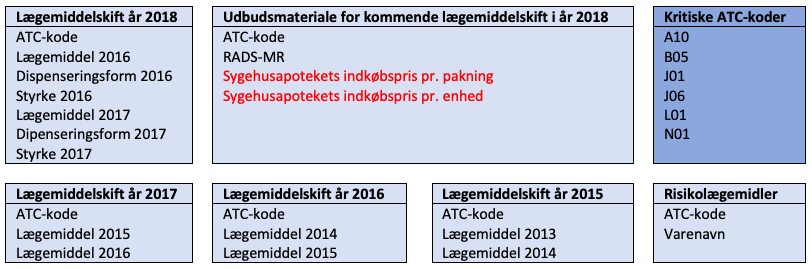
\includegraphics[width=1\textwidth]{billeder/Input.png} 
	\caption{Data anvendt som input til risikovurdering. De lyseblå kasser er data fra forskellige  excel-filer og den mørkeblå kasse data fra en pdf-fil. Teksten angivet med fed refererer til titlen på de enkelte filer.}
	\label{fig:Input}  
\end{figure}



%Data er indsamlet af Amgros og omhandler de aftaler som er indgået i forbindelse med Amgrosudbud. Dette omfatter både forlængelser af allerede eksisterende kontrakter samt ændringer forårsaget af kontraktskift. Sygehusapoteket Region Nordjylland (SRN) udtrækker data fra sygehusapoteksportalen og sorterer i forhold til relevans. Den data der udtrækkes fra sygehusapoteksportalen indeholder alle de aftaler som er indgået, hvorfor det er nødvendigt at sortere indhold for den pågældende udbudsperiode. Denne sortering varetages af en ansat på SRN som udarbejder skiftelister ud fra proceduren, der er beskrevet i Appendiks \ref{cha:AppD} nummer \ref{item:Skiftelister}, hvorefter disse skiftelister sendes ud til de forskellige ATC-ansvarlige, som sortere ud fra ATC-koder i forhold til deres område.

%I dette projekt tages der udgangspunkt i data fra skiftelisterne, som bygger på skiftelister udarbejdet for lægemiddelskift i år 2014-2015(n=231), 2015-2016 (n = 160), 2016-2017 (n=232) og 2017-2018 (n=247). Data indeholder oplysninger om lægemiddelnavn, dispenseringsform og styrke for det fortgående år samt året hvor skiftet skal implementeres. Skiftelisterne kombineres med udtræk fra sygehusapoteksportalen omkring andre forhold som sygehusapotekets indkøbspris per enhed (SAIP/enhed) og oplysninger om hvorvidt lægemiddel er indeholdt i Medicinrådets behandlingsvejledning, hvor der anvendes en deterministisk metode til at matche data. Dette kombineres yderligere med data fra Amgros omhandlende risikolægemidler\fxnote{Overvej om det skal være	Risikosituationslægemidler fra pro.medicin i stedet} og indsamlet data fra SRN omkring kritiske ATC-koder.



%Data er indsamlet af Amgros og Sygehusapoteket Region Nordjylland (SRN) og omhandler lægemiddelskift i år 2018. Data fra Amgros omhandler oplysninger om lægemiddelskiftet foretaget fra år 2017 til 2018. Yderligere har Amgros udarbejdet et dokument over risikolægemidler, som fremgår af Appendiks \ref{cha:AppD}. Risikolægemidler er lægemidler som er særligt risikofyldte hvis disse ender i restordre, da erstatninger er svære at finde samt risikoen for fejl øges ved erstatning. Data fra SRN omhandler de udbud af lægemidler Amgros foretog inden et eventuelt kontraktskift for år 2018. 
%Udover dette har SRN ligeledes indsamlet de problemstillinger der har været vedrørende Amgrosskift siden år 2012.  





%Første trin omhandler identificering af problemer som systemet skal løse, herunder data som systemet skal arbejde på og tilgængelige ressourcer~\citep{Ligeza2006}. Det andet trin er omhandler identificering af nøglekoncepter samt relationer mellem disse som f.eks. typer af data, informationsstrøm og underliggende stukturer. Tredje trin involverer forståelse, beskrivelse og formalisering af problemet og hvordan løsninger findes. Denne proces bør omfatte verificering af systemet. Det fjerde trin har til formål at implementere den formaliseret viden i et program. Det sidste trin omfatter test ved validering af regler og implementeringen.~\citep{Ligeza2006}


\section{Risikofaktorer og vægtning}
Risikofaktorer er udvalgt ud fra den nuværende vurdering af ATC-ansvarlige medarbejdere, som fremgår af Appendiks~\ref{cha:AppD}, punktnummer \ref{item:ATC-ansvarlig}. Litteratur som beskriver risikofaktorer som har ledt til medicineringsfejl i klinikken som følge af lægemiddelskift, hvilket fremgår af Afsnit \ref{sec:ProblemLaeg}. Dokumenterede ATC-koder af SRN, som har ledt til problemstillinger vedrørende lægemiddelskift og derfor anses som kritiske~\citep{SRN}. Lægemidler, der overvåges særligt af Amgros, som er risikofyldte, hvis de ender i restordre på grund af f.eks. leveringesvigt. Liste over risikolægemidler fremgår af Appendiks~\ref{cha:AppD}, punktnummer \ref{item:Risikolaegemidler}. Risikofaktorerne er efter udvælgelsen vægtet af en ekspert inden for området, hvoraf en vægtning på 1 anses som værende af mindre betydning for implementering af lægemiddelskift og 5 anses som værende af stor betydning. Risikofaktorer og deres vægt samt begrundelse for valg fremgår af Tabel \ref{table:features}.

\begin{longtable}{p{3.5cm}| p{1.0cm} | p{9.2cm}}
	\caption{Risikofaktorer} \vspace{0.2cm}
	\label{table:features} \\
\cellcolor[HTML]{C0C0C0} {\textbf{Risikofaktor}} & \cellcolor[HTML]{C0C0C0} {\textbf{Vægt}} & \cellcolor[HTML]{C0C0C0} {\textbf{Begrundelse}} \\ \hline
\textbf{Navn} & 1 & Den hyppigste årsag til medicineringsfejl ved generisk substitution er ordinering af det forkerte lægemiddel, hvilket typisk skyldes at lægemidlets navn lignede og/eller havde et svært navn~\citep{Hakonsen2010}. \\  \hline 
\textbf{Look-a-like} & 2 & Look-a-like har påvist at kunne prædisponeres til medicineringsfejl~\citep{Wittich2014}. Dette kan have patientsikkerhedsmæssige konsekvenser, hvis f.eks. smertestillende panodil forveksles med plendil til behandling af forhøjet blodtryk ~\citep{DanskSelskabforPatientsikkerhed2009}.\\  \hline 
\textbf{Dispenseringsform} & 2 & Dispenseringsform giver anledning til medicineringsfejl i forbindelse med ordination~\citep{Agrawal2009}. Ved ordination af det forkerte lægemiddel, grundet navneforveksling, kan dette give anledning til fejl i dispenseringsform~\citep{DanskSelskabforPatientsikkerhed2009}, hvilket har betydning for virkningen af lægemidlet.
\\ \hline 
\textbf{Styrke} & 2 & Styrke kan medføre medicineringsfejl ved ordination ved f.eks. forkert styrkeberegning~\citep{Agrawal2009}, hvorfor det er vigtigt at være opmærksom på  ændring i styrke for at undgå beregningsfejl, hvormed patienten kan risikere at få en højere eller lavere styrke end ordineret.\\ \hline
\textbf{Risikolægemidler} & 3 & Disse overvåges særligt af Amgros, da de er kritiske hvis de ender i restordre, hvorfor det anbefales at have et lager af disse lægemidler i op til 8 uger~\citep{Amgros}. Yderligere kræver nogle af lægemidlerne et ekstra personalemæssigt ressourcetræk i forbindelse med skift og er i øget risiko for utilsigtede hændelser, som beskrevet i Appendiks ~\ref{cha:AppD}, nummer \ref{item:Risikolaegemidler}  \\ \hline 
\textbf{ATC-grupper} & 5 & ATC-grupper såsom, A10, B05, J01, J06, L01 og N01 har givet anledning til problemstillinger vedrørende lægemiddelskift og er derfor defineret af SRN som kritiske \citep{SRN}.
%står for en stor andel af udgifterne til sygehusmedicin. Over halvdelen af den samlede omsætning er f.eks. til gruppe L som blandt andet inkluderer behandlingen af kræftmedicin, gigtbehandling og sklerose. Andre eksempler er HIV-behandling, øjenbehandlingen og infektioner som er omkostningsfulde.~\citep{Rapport2009}. Da der ofte er store besparelser at opnå ved disse lægemidler skal implementering foregå hurtigt.
 \\ \hline 
\textbf{Medicinråd} & 5 & Lægemidler som indgår i medicinrådets behandlingsvejledninger er lægemidler som er besluttet at anvendes som standardbehandling~\citep{Medicinradet2018}. Disse vurderes i forhold til effekt, eksisterende behandling og pris~\citep{Medicinradet2018}. For lægemidler som indgår i Medicinrådet er der ofte mange penge og spare, hvorfor disse skal implementeres hurtigt. \\ \hline 
\textbf{Pris} &  2 & \textcolor{red}{ IKKE BESLUTTET ENDNU Pris er vigtigt i forhold til at opnå besparelser. Det skal ligeledes vægtes om det kan betale sig at skifte et lægemiddel med mindre besparelse, da udskiftningen kan få store betydninger for klinikken i forhold til arbejdsgangen og i værste tilfælde medføre patientsikkerhedsmæssige konsekvenser. [KILDE, AMGROS]} \\ \hline
    \end{longtable}

\section{Præprocessering}
Præprocessering af data er nødvendigt, da data er tekstbaseret og indskrevet manuelt og derfor ikke sammenligneligt. Det er forskelligt om data er skrevet med majuskel eller minuskel, hvorfor det er valgt at ændre alt data til minuskel. Ligeledes er forkortelser udskrevet og tegnsætning fjernet for at gøre data generaliserbar. 

Det antages at lægemiddelnavne er ens, hvis deres præfiks er uændret, hvorfor suffiks er fjernet. Lægemidler med ens præfiks, men forskellig suffiks, kan have anderledes dispenseringsform eller styrke. Dette forventes dog at opdages i forbindelse med sammenligning af dispenseringsform og styrke. Det er for dispenseringsformer antaget at filmovertrukne tabelletter er det samme som tabelletter og hvis ingen dispenseringsform er angivet er denne uændret.

\section{Design}
\textcolor{red}{Tilføj: Hvilke overvejelser har jeg gjort i design i forhold til at gøre systemet generealiserbart?} \\
Risikovurderingen er designet som if-then-else statements som danner grundlag for risikovurderingen. For hvert statement vurderes én eller flere risikofaktorer i forhold til om et statement er sandt eller falsk. Ud fra antallet af sande statements beregnes risikoscoren ud fra Ligning \ref{equ:risikoscore} på baggrund af den totale vægt af alle matchende risikofaktorer og den totale vægt af alle risikofaktorer.

\begin{equation}  \label{equ:risikoscore}
Riskoscore = \frac{\mbox{\textit{Totale vægt af alle matchende risikofaktorer}}}{\mbox{\textit{Totale vægt af alle risikofaktorer}}} * 100
\end{equation}

Risikoscoren er angivet som en procentdel. En  høj risikoscore vil betyde at de risikofaktorer som gør sig gældende har en stor betydning for implementering af lægemiddelskift. Hvis risikoscoren modsat er lille vil dette have en mindre betydning for implementering af lægemiddelskift. Det skal på denne måde være muligt for de ATC-ansvarlige medarbejdere på SRN at skelne hvilke tilfælde de skal være ekstra opmærksomme på lægemiddelskift i forhold til udarbejdelsen af Lægemiddel Nyt.  

Til design af look-a-like lægemidler, som sammenligner, hvorvidt et lægemiddelnavn fra år 2017 ligner et allerede eksisterende lægemiddelnavn fra år 2013 til 2016, beregnes Levenshtein distance. Levenshtein distance er et udtryk for det minimale antal af operationer, herunder slette, indføre eller erstatte, der kræves for at ændre et ord til et andet. Denne distance beregnes ud fra Ligning \ref{equ:LevDistance} på baggrund af det minimale antal af tilføjede, slettede og erstattede bogstaver der kræves for at ændre et ord til et andet samt den maksimale længde af de to ord som sammenlignes. 

\begin{equation} \label{equ:LevDistance}
\mbox{\textit{Distance}} = 1 - \frac{\mbox{\textit{min(antal af tilføjede, slettede og erstattede bogstaver)}}}{\mbox{\textit{max(længde af ord der sammenlinges)}}}   
\end{equation}

\fxnote{måske tilføje hvordan jeg vurdere hvornår antallet af operationer er højt eller lavt?}

Outputtet er designet ud fra det excelark som anvendes på nuværende tidspunkt af de ATC-ansvarlige medarbejdere. Udover de nuværende data tilføjes en ekstra kolonne til excelarket, som indeholder risikoscore og grundlag for denne score. Designet af outputtet fremgår af Figur \ref{fig:Output}.

\begin{figure}[H]\centering
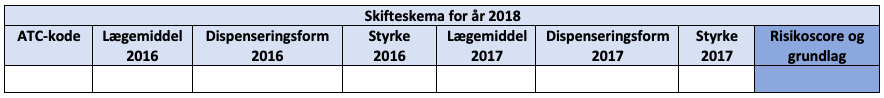
\includegraphics[width=1\textwidth]{billeder/Output.png} 
	\caption{Design af output. De lyseblå kasser illustrerer de eksisterende excel kolonner i excelarket, hvor den mørkeblå kasse illusterer en ektra kolonne som indeholder risikoscore samt grundlaget for denne.}
	\label{fig:Output}  
\end{figure}

%\begin{equation} \label{eq1}
%\begin{split}
%Risikoscore = lægemiddelnavn + ligende lægemiddelnavn + dispenseringsform \\ 
%+ styrke + medicnråd + risikolægemiddel + kritisk ATC-kode \\
%+ pris
%\end{split}
%\end{equation}

\section{Implementering og test}
\textcolor{red}{Måske reference til kode i appendiks, når koden er helt færdig} \\
Systemet er implementeret i NetBeans, som er et Integrated Development Environment (IDE) til java. For at kunne håndtere Microsoft dokumenter blev Java Excel API (JExcelApi) og Apache POI tilføjet til biblioteket. Tegnsættet blev ændret til ISO-8859-15 i NetBeans IDE for at kunne håndtere æ, ø og å. 

Enkelte dele af systemet blev efter implementeringen løbende testet og valideret i forhold til at undersøge om systemet performer efter formålet. Hvis dette ikke var tilfældet blev de enkelte dele af systemet tilpasset i koden, hvorefter disse blev testet igen indtil systemet performans var acceptabel.

\section{Evaluering}
\textcolor{red}{Skriv mere til når det er mere klart, hvordan dette kommer til at forløbe.} \\
Systemet evalueres for at undersøge anvendeligheden af systemet samt, hvorvidt et system som dette vil kunne forbedre arbejdsgangen for ATC-ansvarlige medarbejdere vedrørende lægemiddelskift. Dette gøres i et gruppeinterview med ATC-ansvarlige medarbejdere på SRN. I denne evaluering vurderes outputtet fra systemet herunder risikoscore samt grundlaget for beregningen af risikoscoren. 
Derudover diskuteres forbedringer af systemet med henblik på videreudvikling af systemet.




